%% bare_jrnl.tex
%% V1.3
%% 2007/01/11
%% by Michael Shell
%% see http://www.michaelshell.org/
%% for current contact information.
%%
%% This is a skeleton file demonstrating the use of IEEEtran.cls
%% (requires IEEEtran.cls version 1.7 or later) with an IEEE journal paper.
%%
%% Support sites:
%% http://www.michaelshell.org/tex/ieeetran/
%% http://www.ctan.org/tex-archive/macros/latex/contrib/IEEEtran/
%% and
%% http://www.ieee.org/



% *** Authors should verify (and, if needed, correct) their LaTeX system  ***
% *** with the testflow diagnostic prior to trusting their LaTeX platform ***
% *** with production work. IEEE's font choices can trigger bugs that do  ***
% *** not appear when using other class files.                            ***
% The testflow support page is at:
% http://www.michaelshell.org/tex/testflow/


%%*************************************************************************
%% Legal Notice:
%% This code is offered as-is without any warranty either expressed or
%% implied; without even the implied warranty of MERCHANTABILITY or
%% FITNESS FOR A PARTICULAR PURPOSE! 
%% User assumes all risk.
%% In no event shall IEEE or any contributor to this code be liable for
%% any damages or losses, including, but not limited to, incidental,
%% consequential, or any other damages, resulting from the use or misuse
%% of any information contained here.
%%
%% All comments are the opinions of their respective authors and are not
%% necessarily endorsed by the IEEE.
%%
%% This work is distributed under the LaTeX Project Public License (LPPL)
%% ( http://www.latex-project.org/ ) version 1.3, and may be freely used,
%% distributed and modified. A copy of the LPPL, version 1.3, is included
%% in the base LaTeX documentation of all distributions of LaTeX released
%% 2003/12/01 or later.
%% Retain all contribution notices and credits.
%% ** Modified files should be clearly indicated as such, including  **
%% ** renaming them and changing author support contact information. **
%%
%% File list of work: IEEEtran.cls, IEEEtran_HOWTO.pdf, bare_adv.tex,
%%                    bare_conf.tex, bare_jrnl.tex, bare_jrnl_compsoc.tex
%%*************************************************************************

% Note that the a4paper option is mainly intended so that authors in
% countries using A4 can easily print to A4 and see how their papers will
% look in print - the typesetting of the document will not typically be
% affected with changes in paper size (but the bottom and side margins will).
% Use the testflow package mentioned above to verify correct handling of
% both paper sizes by the user's LaTeX system.
%
% Also note that the "draftcls" or "draftclsnofoot", not "draft", option
% should be used if it is desired that the figures are to be displayed in
% draft mode.
%
\documentclass[conference, a4paper]{IEEEtran}
\IEEEoverridecommandlockouts
%
% If IEEEtran.cls has not been installed into the LaTeX system files,
% manually specify the path to it like:
% \documentclass[journal]{../sty/IEEEtran}


\usepackage[utf8]{inputenc}
\usepackage{todonotes}
\newcommand{\todonote}[2][]{\todo[size=\tiny, #1]{#2}}
\newcommand{\quotes}[1]{``#1''} 


% Some very useful LaTeX packages include:
% (uncomment the ones you want to load)


% *** MISC UTILITY PACKAGES ***
%
%\usepackage{ifpdf}
% Heiko Oberdiek's ifpdf.sty is very useful if you need conditional
% compilation based on whether the output is pdf or dvi.
% usage:
% \ifpdf
%   % pdf code
% \else
%   % dvi code
% \fi
% The latest version of ifpdf.sty can be obtained from:
% http://www.ctan.org/tex-archive/macros/latex/contrib/oberdiek/
% Also, note that IEEEtran.cls V1.7 and later provides a builtin
% \ifCLASSINFOpdf conditional that works the same way.
% When switching from latex to pdflatex and vice-versa, the compiler may
% have to be run twice to clear warning/error messages.






% *** CITATION PACKAGES ***
%
%\usepackage{cite}
% cite.sty was written by Donald Arseneau
% V1.6 and later of IEEEtran pre-defines the format of the cite.sty package
% \cite{} output to follow that of IEEE. Loading the cite package will
% result in citation numbers being automatically sorted and properly
% "compressed/ranged". e.g., [1], [9], [2], [7], [5], [6] without using
% cite.sty will become [1], [2], [5]--[7], [9] using cite.sty. cite.sty's
% \cite will automatically add leading space, if needed. Use cite.sty's
% noadjust option (cite.sty V3.8 and later) if you want to turn this off.
% cite.sty is already installed on most LaTeX systems. Be sure and use
% version 4.0 (2003-05-27) and later if using hyperref.sty. cite.sty does
% not currently provide for hyperlinked citations.
% The latest version can be obtained at:
% http://www.ctan.org/tex-archive/macros/latex/contrib/cite/
% The documentation is contained in the cite.sty file itself.






% *** GRAPHICS RELATED PACKAGES ***
%
\ifCLASSINFOpdf
  % \usepackage[pdftex]{graphicx}
  % declare the path(s) where your graphic files are
  % \graphicspath{{../pdf/}{../jpeg/}}
  % and their extensions so you won't have to specify these with
  % every instance of \includegraphics
  % \DeclareGraphicsExtensions{.pdf,.jpeg,.png}
\else
  % or other class option (dvipsone, dvipdf, if not using dvips). graphicx
  % will default to the driver specified in the system graphics.cfg if no
  % driver is specified.
  % \usepackage[dvips]{graphicx}
  % declare the path(s) where your graphic files are
  % \graphicspath{{../eps/}}
  % and their extensions so you won't have to specify these with
  % every instance of \includegraphics
  % \DeclareGraphicsExtensions{.eps}
\fi
% graphicx was written by David Carlisle and Sebastian Rahtz. It is
% required if you want graphics, photos, etc. graphicx.sty is already
% installed on most LaTeX systems. The latest version and documentation can
% be obtained at: 
% http://www.ctan.org/tex-archive/macros/latex/required/graphics/
% Another good source of documentation is "Using Imported Graphics in
% LaTeX2e" by Keith Reckdahl which can be found as epslatex.ps or
% epslatex.pdf at: http://www.ctan.org/tex-archive/info/
%
% latex, and pdflatex in dvi mode, support graphics in encapsulated
% postscript (.eps) format. pdflatex in pdf mode supports graphics
% in .pdf, .jpeg, .png and .mps (metapost) formats. Users should ensure
% that all non-photo figures use a vector format (.eps, .pdf, .mps) and
% not a bitmapped formats (.jpeg, .png). IEEE frowns on bitmapped formats
% which can result in "jaggedy"/blurry rendering of lines and letters as
% well as large increases in file sizes.
%
% You can find documentation about the pdfTeX application at:
% http://www.tug.org/applications/pdftex





% *** MATH PACKAGES ***
%
%\usepackage[cmex10]{amsmath}
% A popular package from the American Mathematical Society that provides
% many useful and powerful commands for dealing with mathematics. If using
% it, be sure to load this package with the cmex10 option to ensure that
% only type 1 fonts will utilized at all point sizes. Without this option,
% it is possible that some math symbols, particularly those within
% footnotes, will be rendered in bitmap form which will result in a
% document that can not be IEEE Xplore compliant!
%
% Also, note that the amsmath package sets \interdisplaylinepenalty to 10000
% thus preventing page breaks from occurring within multiline equations. Use:
%\interdisplaylinepenalty=2500
% after loading amsmath to restore such page breaks as IEEEtran.cls normally
% does. amsmath.sty is already installed on most LaTeX systems. The latest
% version and documentation can be obtained at:
% http://www.ctan.org/tex-archive/macros/latex/required/amslatex/math/





% *** SPECIALIZED LIST PACKAGES ***
%
%\usepackage{algorithmic}
% algorithmic.sty was written by Peter Williams and Rogerio Brito.
% This package provides an algorithmic environment fo describing algorithms.
% You can use the algorithmic environment in-text or within a figure
% environment to provide for a floating algorithm. Do NOT use the algorithm
% floating environment provided by algorithm.sty (by the same authors) or
% algorithm2e.sty (by Christophe Fiorio) as IEEE does not use dedicated
% algorithm float types and packages that provide these will not provide
% correct IEEE style captions. The latest version and documentation of
% algorithmic.sty can be obtained at:
% http://www.ctan.org/tex-archive/macros/latex/contrib/algorithms/
% There is also a support site at:
% http://algorithms.berlios.de/index.html
% Also of interest may be the (relatively newer and more customizable)
% algorithmicx.sty package by Szasz Janos:
% http://www.ctan.org/tex-archive/macros/latex/contrib/algorithmicx/




% *** ALIGNMENT PACKAGES ***
%
%\usepackage{array}
% Frank Mittelbach's and David Carlisle's array.sty patches and improves
% the standard LaTeX2e array and tabular environments to provide better
% appearance and additional user controls. As the default LaTeX2e table
% generation code is lacking to the point of almost being broken with
% respect to the quality of the end results, all users are strongly
% advised to use an enhanced (at the very least that provided by array.sty)
% set of table tools. array.sty is already installed on most systems. The
% latest version and documentation can be obtained at:
% http://www.ctan.org/tex-archive/macros/latex/required/tools/


%\usepackage{mdwmath}
%\usepackage{mdwtab}
% Also highly recommended is Mark Wooding's extremely powerful MDW tools,
% especially mdwmath.sty and mdwtab.sty which are used to format equations
% and tables, respectively. The MDWtools set is already installed on most
% LaTeX systems. The lastest version and documentation is available at:
% http://www.ctan.org/tex-archive/macros/latex/contrib/mdwtools/


% IEEEtran contains the IEEEeqnarray family of commands that can be used to
% generate multiline equations as well as matrices, tables, etc., of high
% quality.


%\usepackage{eqparbox}
% Also of notable interest is Scott Pakin's eqparbox package for creating
% (automatically sized) equal width boxes - aka "natural width parboxes".
% Available at:
% http://www.ctan.org/tex-archive/macros/latex/contrib/eqparbox/





% *** SUBFIGURE PACKAGES ***
%\usepackage[tight,footnotesize]{subfigure}
% subfigure.sty was written by Steven Douglas Cochran. This package makes it
% easy to put subfigures in your figures. e.g., "Figure 1a and 1b". For IEEE
% work, it is a good idea to load it with the tight package option to reduce
% the amount of white space around the subfigures. subfigure.sty is already
% installed on most LaTeX systems. The latest version and documentation can
% be obtained at:
% http://www.ctan.org/tex-archive/obsolete/macros/latex/contrib/subfigure/
% subfigure.sty has been superceeded by subfig.sty.



%\usepackage[caption=false]{caption}
%\usepackage[font=footnotesize]{subfig}
% subfig.sty, also written by Steven Douglas Cochran, is the modern
% replacement for subfigure.sty. However, subfig.sty requires and
% automatically loads Axel Sommerfeldt's caption.sty which will override
% IEEEtran.cls handling of captions and this will result in nonIEEE style
% figure/table captions. To prevent this problem, be sure and preload
% caption.sty with its "caption=false" package option. This is will preserve
% IEEEtran.cls handing of captions. Version 1.3 (2005/06/28) and later 
% (recommended due to many improvements over 1.2) of subfig.sty supports
% the caption=false option directly:
%\usepackage[caption=false,font=footnotesize]{subfig}
%
% The latest version and documentation can be obtained at:
% http://www.ctan.org/tex-archive/macros/latex/contrib/subfig/
% The latest version and documentation of caption.sty can be obtained at:
% http://www.ctan.org/tex-archive/macros/latex/contrib/caption/




% *** FLOAT PACKAGES ***
%
%\usepackage{fixltx2e}
% fixltx2e, the successor to the earlier fix2col.sty, was written by
% Frank Mittelbach and David Carlisle. This package corrects a few problems
% in the LaTeX2e kernel, the most notable of which is that in current
% LaTeX2e releases, the ordering of single and double column floats is not
% guaranteed to be preserved. Thus, an unpatched LaTeX2e can allow a
% single column figure to be placed prior to an earlier double column
% figure. The latest version and documentation can be found at:
% http://www.ctan.org/tex-archive/macros/latex/base/



%\usepackage{stfloats}
% stfloats.sty was written by Sigitas Tolusis. This package gives LaTeX2e
% the ability to do double column floats at the bottom of the page as well
% as the top. (e.g., "\begin{figure*}[!b]" is not normally possible in
% LaTeX2e). It also provides a command:
%\fnbelowfloat
% to enable the placement of footnotes below bottom floats (the standard
% LaTeX2e kernel puts them above bottom floats). This is an invasive package
% which rewrites many portions of the LaTeX2e float routines. It may not work
% with other packages that modify the LaTeX2e float routines. The latest
% version and documentation can be obtained at:
% http://www.ctan.org/tex-archive/macros/latex/contrib/sttools/
% Documentation is contained in the stfloats.sty comments as well as in the
% presfull.pdf file. Do not use the stfloats baselinefloat ability as IEEE
% does not allow \baselineskip to stretch. Authors submitting work to the
% IEEE should note that IEEE rarely uses double column equations and
% that authors should try to avoid such use. Do not be tempted to use the
% cuted.sty or midfloat.sty packages (also by Sigitas Tolusis) as IEEE does
% not format its papers in such ways.


%\ifCLASSOPTIONcaptionsoff
%  \usepackage[nomarkers]{endfloat}
% \let\MYoriglatexcaption\caption
% \renewcommand{\caption}[2][\relax]{\MYoriglatexcaption[#2]{#2}}
%\fi
% endfloat.sty was written by James Darrell McCauley and Jeff Goldberg.
% This package may be useful when used in conjunction with IEEEtran.cls'
% captionsoff option. Some IEEE journals/societies require that submissions
% have lists of figures/tables at the end of the paper and that
% figures/tables without any captions are placed on a page by themselves at
% the end of the document. If needed, the draftcls IEEEtran class option or
% \CLASSINPUTbaselinestretch interface can be used to increase the line
% spacing as well. Be sure and use the nomarkers option of endfloat to
% prevent endfloat from "marking" where the figures would have been placed
% in the text. The two hack lines of code above are a slight modification of
% that suggested by in the endfloat docs (section 8.3.1) to ensure that
% the full captions always appear in the list of figures/tables - even if
% the user used the short optional argument of \caption[]{}.
% IEEE papers do not typically make use of \caption[]'s optional argument,
% so this should not be an issue. A similar trick can be used to disable
% captions of packages such as subfig.sty that lack options to turn off
% the subcaptions:
% For subfig.sty:
% \let\MYorigsubfloat\subfloat
% \renewcommand{\subfloat}[2][\relax]{\MYorigsubfloat[]{#2}}
% For subfigure.sty:
% \let\MYorigsubfigure\subfigure
% \renewcommand{\subfigure}[2][\relax]{\MYorigsubfigure[]{#2}}
% However, the above trick will not work if both optional arguments of
% the \subfloat/subfig command are used. Furthermore, there needs to be a
% description of each subfigure *somewhere* and endfloat does not add
% subfigure captions to its list of figures. Thus, the best approach is to
% avoid the use of subfigure captions (many IEEE journals avoid them anyway)
% and instead reference/explain all the subfigures within the main caption.
% The latest version of endfloat.sty and its documentation can obtained at:
% http://www.ctan.org/tex-archive/macros/latex/contrib/endfloat/
%
% The IEEEtran \ifCLASSOPTIONcaptionsoff conditional can also be used
% later in the document, say, to conditionally put the References on a 
% page by themselves.





% *** PDF, URL AND HYPERLINK PACKAGES ***
%
%\usepackage{url}
% url.sty was written by Donald Arseneau. It provides better support for
% handling and breaking URLs. url.sty is already installed on most LaTeX
% systems. The latest version can be obtained at:
% http://www.ctan.org/tex-archive/macros/latex/contrib/misc/
% Read the url.sty source comments for usage information. Basically,
% \url{my_url_here}.





% *** Do not adjust lengths that control margins, column widths, etc. ***
% *** Do not use packages that alter fonts (such as pslatex).         ***
% There should be no need to do such things with IEEEtran.cls V1.6 and later.
% (Unless specifically asked to do so by the journal or conference you plan
% to submit to, of course. )


% correct bad hyphenation here
\hyphenation{op-tical net-works semi-conduc-tor}


\begin{document}
\urlstyle{tt}
%
% paper title
% can use linebreaks \\ within to get better formatting as desired
\title{Applying Model-View-Presenter Architecture to the Android Framework with App Prototype}
%
%
% author names and IEEE memberships
% note positions of commas and nonbreaking spaces ( ~ ) LaTeX will not break
% a structure at a ~ so this keeps an author's name from being broken across
% two lines.
% use \thanks{} to gain access to the first footnote area
% a separate \thanks must be used for each paragraph as LaTeX2e's \thanks
% was not built to handle multiple paragraphs
%

%\author{Dennis~G.~Geisse\\dennis\gregor.geisse@student.reutlingen-university.de \and Iven~John\\iven.john@student.reutlingen-university.de \and Daniel~Joos\\daniel.joos@student.reutlingen-university.de \and Sebastian~Kotstein\\sebastian.kotstein@student.reutlingen-university.de \and Michael~Wurster\\michael.wurster@student.reutlingen-university.de}

%\author{
%\IEEEauthorblockN{Dennis~G.~Geisse}
%\IEEEauthorblockA{Reutlingen University\\
%dennis\_gregor.geisse@student.reutlingen-university.de}
%\\
%\IEEEauthorblockN{Iven~John}
%\IEEEauthorblockA{Reutlingen University\\
%iven.john@student.reutlingen-university.de}
%\and 
%\IEEEauthorblockN{Daniel~Joos}
%\IEEEauthorblockA{Reutlingen University\\
%daniel.joos@student.reutlingen-university.de}
%\and 
%\IEEEauthorblockN{Sebastian~Kotstein}
%\IEEEauthorblockA{Reutlingen University\\
%sebastian.kotstein@student.reutlingen-university.de}
%\\\
%\IEEEauthorblockN{Michael~Wurster}
%\IEEEauthorblockA{Reutlingen University\\
%michael.wurster@student.reutlingen-university.de}
%}

\author{
\IEEEauthorblockN{Dennis~G.~Geisse, Iven~John, Daniel~Joos, Sebastian~Kotstein, Michael~Wurster}
\IEEEauthorblockA{Reutlingen University, Hermann Hollerith Zentrum\\
Email: [dennis\_gregor.geisse, iven.john, daniel.joos, sebastian.kotstein, michael.wurster]@student.reutlingen-university.de}
}

% note the % following the last \IEEEmembership and also \thanks - 
% these prevent an unwanted space from occurring between the last author name
% and the end of the author line. i.e., if you had this:
% 
% \author{....lastname \thanks{...} \thanks{...} }
%                     ^------------^------------^----Do not want these spaces!
%
% a space would be appended to the last name and could cause every name on that
% line to be shifted left slightly. This is one of those "LaTeX things". For
% instance, "\textbf{A} \textbf{B}" will typeset as "A B" not "AB". To get
% "AB" then you have to do: "\textbf{A}\textbf{B}"
% \thanks is no different in this regard, so shield the last } of each \thanks
% that ends a line with a % and do not let a space in before the next \thanks.
% Spaces after \IEEEmembership other than the last one are OK (and needed) as
% you are supposed to have spaces between the names. For what it is worth,
% this is a minor point as most people would not even notice if the said evil
% space somehow managed to creep in.



% The paper headers
\markboth{Geisse, John, Joos, Kotstein, Wurster (2015)}%
{Software Architecture,~Hermann Hollerith Zentrum,~January~2015}
% The only time the second header will appear is for the odd numbered pages
% after the title page when using the twoside option.
% 
% *** Note that you probably will NOT want to include the author's ***
% *** name in the headers of peer review papers.                   ***
% You can use \ifCLASSOPTIONpeerreview for conditional compilation here if
% you desire.




% If you want to put a publisher's ID mark on the page you can do it like
% this:
%\IEEEpubid{0000--0000/00\$00.00~\copyright~2007 IEEE}
% Remember, if you use this you must call \IEEEpubidadjcol in the second
% column for its text to clear the IEEEpubid mark.



% use for special paper notices
%\IEEEspecialpapernotice{(Invited Paper)}




% make the title area
\maketitle


\begin{abstract}
%\boldmath
Minions ipsum me want bananaaa! Hahaha chasy hana dul sae belloo! Aaaaaah daa ti aamoo! La bodaaa pepete. La bodaaa para tú gelatooo underweaaar po kass tank yuuu! Underweaaar. Wiiiii bappleees jiji chasy underweaaar. Tank yuuu! jeje me want bananaaa! Me want bananaaa! Hahaha aaaaaah chasy hana dul sae gelatooo jeje tulaliloo. Baboiii bappleees wiiiii daa underweaaar tank yuuu! Underweaaar. Jiji potatoooo butt la bodaaa ti aamoo! Para tú tatata bala tu. Jiji underweaaar bappleees belloo! La bodaaa. Bee do bee do bee do jiji tatata bala tu belloo! Gelatooo bappleees hana dul sae ti aamoo!

Poopayee bappleees underweaaar bee do bee do bee do. Hana dul sae potatoooo bappleees la bodaaa baboiii. Pepete para tú hana dul sae tank yuuu! Jiji poulet tikka masala tatata bala tu ti aamoo! Po kass belloo! Wiiiii daa me want bananaaa! Chasy poopayee jeje po kass.
\end{abstract}
% IEEEtran.cls defaults to using nonbold math in the Abstract.
% This preserves the distinction between vectors and scalars. However,
% if the journal you are submitting to favors bold math in the abstract,
% then you can use LaTeX's standard command \boldmath at the very start
% of the abstract to achieve this. Many IEEE journals frown on math
% in the abstract anyway.

% Note that keywords are not normally used for peerreview papers.
\begin{IEEEkeywords}
Android,  Application Architecture, Model-View-Presenter (MVP), App Prototype.
\end{IEEEkeywords}






% For peer review papers, you can put extra information on the cover
% page as needed:
% \ifCLASSOPTIONpeerreview
% \begin{center} \bfseries EDICS Category: 3-BBND \end{center}
% \fi
%
% For peerreview papers, this IEEEtran command inserts a page break and
% creates the second title. It will be ignored for other modes.
\IEEEpeerreviewmaketitle



\section{Introduction}

\IEEEPARstart{T}{he \emph{Android}} operating system is one of the most 
commonly used in mobile industry. After its first presentation in 2007, the open source system started its successful journey and became the leading mobile operating system in 2010 \cite{PassiveMVC}. According to Gartner \cite{GartnerAndroid2014}, there will be 1.1 billion \emph{Android}-based devices sold in 2014.

What brings the actual value to an \emph{Android} device is the installed software, the so called \quotes{Applications} or 
\quotes{Apps}.
Software for \emph{Android} devices can be downloaded and installed via the 
\emph{Play Store}, a software distribution solution, developed by Google and 
pre-installed on every new device, which currently holds over 1.4 million 
applications (as of November 2014) \cite{AppBrainStats}.\\

%\subsection{Application Development}

For developing such an application for the \emph{Android} mobile operating 
system, Google provides a software development kit (SDK) for the programming 
language \emph{Java}. It provides access to all functionality of the 
operating system and the underlaying phone- or tablet hardware. The principle components of the \emph{Android} SDK are explained later in this document.\\

%\subsection{Challenges in Android Development}

The SDK does not define a specific software architecture which has to 
be used for developing the application \cite{AndroidDeveloperCollection}. Instead, developers are totally free in 
designing their own architecture for fitting their needs for an application.
Having the number of 1.4 million applications in mind, this fact implies that 
there are various different software architectures currently implemented, each 
of them with their pros and cons. 

However, not having clear rules regarding the application's architecture entails risks, especially for people that are not expert-level developers. Applications become larger from time to time, and without a reasonable architecture this leads to complex code which is hard to understand and maintain \cite{PassiveMVC, BallOfMud}. Additionally, complex dependencies in the SDK cause messy code and make it hard to exchange specific elements without affecting other elements \cite{PassiveMVC}. That is especially because \emph{Android} tends to lead to classes containing a lot of functionality, which often requires more effort concerning testability and extendability \cite{GangOfFour}. \\

%\subsection{Model-View-Presenter Architecture}

A modern architecture approach is Model-View-Presenter (MVP), a model introduced in 1996 to support event-driven systems \cite{TaligentMVP}. Its main goal is to separate the data logic from the presentation logic, thus creating software which is more flexible in terms of replacing the data model without changing the presentation part or vice versa \cite{PassiveMVC}. Therefor, the software is split into three parts: The \emph{Model} provides the data and means to manipulate it, the \emph{View} part is responsible to display the data, and the \emph{Presenter} contains the business logic that handles user-initiated events and issues the appropriate manipulation of the data \cite{TaligentMVP}.\\

%\subsection{Applying MVP in Android}

Applying MVP to \emph{Android} applications seems promising to build less complex applications with clear code and improved extensibility. However, as the considerations in this paper show, an \emph{Android} implementation of MVP is tricky. Some components of the SDK have several responsibilities and make it hard to define whether they are a \emph{Model}, a \emph{View} or a \emph{Presenter} \cite{PassiveMVC}. 

The approach developed in this paper aims to clarify the distinction of these architectural parts. The findings of our research may serve as a guideline on how to apply MVP in \emph{Android} application development.\\

%\subsection{Research Questions}
In the following sections, these questions concerning the application of MVP to \emph{Android} application development are evaluated and answered:

\begin{enumerate}[label={RQ\arabic*:}, leftmargin=0.95cm]
\item What are the inherent characteristics given / recommended by the Android Framework? What is the current state in Android Development in accordance to the inherent framework characteristics?
\item What are the key benefits of the Model-View-Presenter approach?
\item How can the MVP model be applied to the Android App architecture considering framework building blocks?
\end{enumerate}

To answer these questions, a prototypical App is built using the MVP approach.
\todo[inline]{Outlook for each chapter?}




% An example of a floating figure using the graphicx package.
% Note that \label must occur AFTER (or within) \caption.
% For figures, \caption should occur after the \includegraphics.
% Note that IEEEtran v1.7 and later has special internal code that
% is designed to preserve the operation of \label within \caption
% even when the captionsoff option is in effect. However, because
% of issues like this, it may be the safest practice to put all your
% \label just after \caption rather than within \caption{}.
%
% Reminder: the "draftcls" or "draftclsnofoot", not "draft", class
% option should be used if it is desired that the figures are to be
% displayed while in draft mode.
%
%\begin{figure}[!t]
%\centering
%\includegraphics[width=2.5in]{myfigure}
% where an .eps filename suffix will be assumed under latex, 
% and a .pdf suffix will be assumed for pdflatex; or what has been declared
% via \DeclareGraphicsExtensions.
%\caption{Simulation Results}
%\label{fig_sim}
%\end{figure}

% Note that IEEE typically puts floats only at the top, even when this
% results in a large percentage of a column being occupied by floats.


% An example of a double column floating figure using two subfigures.
% (The subfig.sty package must be loaded for this to work.)
% The subfigure \label commands are set within each subfloat command, the
% \label for the overall figure must come after \caption.
% \hfil must be used as a separator to get equal spacing.
% The subfigure.sty package works much the same way, except \subfigure is
% used instead of \subfloat.
%
%\begin{figure*}[!t]
%\centerline{\subfloat[Case I]\includegraphics[width=2.5in]{subfigcase1}%
%\label{fig_first_case}}
%\hfil
%\subfloat[Case II]{\includegraphics[width=2.5in]{subfigcase2}%
%\label{fig_second_case}}}
%\caption{Simulation results}
%\label{fig_sim}
%\end{figure*}
%
% Note that often IEEE papers with subfigures do not employ subfigure
% captions (using the optional argument to \subfloat), but instead will
% reference/describe all of them (a), (b), etc., within the main caption.


% An example of a floating table. Note that, for IEEE style tables, the 
% \caption command should come BEFORE the table. Table text will default to
% \footnotesize as IEEE normally uses this smaller font for tables.
% The \label must come after \caption as always.
%
%\begin{table}[!t]
%% increase table row spacing, adjust to taste
%\renewcommand{\arraystretch}{1.3}
% if using array.sty, it might be a good idea to tweak the value of
% \extrarowheight as needed to properly center the text within the cells
%\caption{An Example of a Table}
%\label{table_example}
%\centering
%% Some packages, such as MDW tools, offer better commands for making tables
%% than the plain LaTeX2e tabular which is used here.
%\begin{tabular}{|c||c|}
%\hline
%One & Two\\
%\hline
%Three & Four\\
%\hline
%\end{tabular}
%\end{table}


% Note that IEEE does not put floats in the very first column - or typically
% anywhere on the first page for that matter. Also, in-text middle ("here")
% positioning is not used. Most IEEE journals use top floats exclusively.
% Note that, LaTeX2e, unlike IEEE journals, places footnotes above bottom
% floats. This can be corrected via the \fnbelowfloat command of the
% stfloats package.

\section{Research}
\label{sec:research}
\IEEEPARstart{B}{efore} the application prototype is built, composing components of \emph{Android} applications are introduced in this chapter. In addition, it is shown why the MVP approach may improve app development and what MVP actually is.
% MVP applied to Android Apps

\subsection{Concepts \& Components of Android Applications}
Building \emph{Android} applications requires several core components of the \emph{Android} SDK to be used. This section gives a short overview and explanation of important components used in the implementation of the prototype created for this paper.

\textbf{Activity}: An application typically consists of one or more activities. An activity fills the whole screen of the device and can be compared to a \emph{window} in a classic desktop application. The official \emph{Android} SDK documentation \cite{SDKActivities} defines an activity as \enquote{an application component that provides a screen with which users can interact in order to do something}.
There is a defined lifcycle, which all activity objects share and follow -- the creation, start, resume, pause, stop and the destruction of an activity object. This lifecycle is managed by \emph{Android} itself, meaning application developers must not manually create or destroy activity objects.

\textbf{Fragment}: Fragments split more complex parts of an activity's user interface into several smaller sub-components. Fragments are also used to encapsulate reusable parts of the user interface, which for example need to appear in multiple activities. The official documentation of the \emph{Android} SDK defines a fragment as follows \cite{SDKFragments}:

\begin{quote}
A Fragment represents a behavior or a portion of user interface in an Activity. You can combine multiple fragments in a single activity to build a multi-pane UI and reuse a fragment in multiple activities.
\end{quote}

\textbf{Intent}: Intents are objects used for communication with the \emph{Android} system. An example would be the start of an activity: an intent must be created including some information to identify, which activity should be started. The intent will be handed over to the \emph{Android} system, which will create and start a corresponding activity. In the official SDK documentation, an intent is defined as \enquote{a messaging object you can use to request an action from another app component} \cite{SDKIntents}.

\subsection{Common Android Development Approach}
As a result of strong interrelations between its building components, the \emph{Android} system manages most of its components by itself. Given the complexity and interaction between these as well as the general structure, the framework steers developers toward handling tasks in common ways. In order to help developers understand the structure of the framework, code examples and component explanations are provided in \cite{SDKComponents}.

Since the building components are managed by the system and dependent on the implementations, one aspect that is inherently difficult is \emph{testability}. It is a challenge to divide business logic from the framework as it needs to react to certain system events -- like activity destruction, which may be forced by the system at any point in time and need to be appropriately handled by the developer.

Other common difficulties developers face lie with the \emph{maintainability} and \emph{extensibility} of their software. Given the \emph{Android} framework, its many components and classes that enable communication between these components, the structure often gets cluttered -- especially in larger application projects. For example, \emph{ListView}s\footnote{Component to \enquote{display a list of scrollable items} \cite{SDKListView}.} need \emph{Adapter}\footnote{Class to \enquote{bridge between AdapterView and the underlying data} \cite{SDKAdapter}.} to display their content, which in turn might use \emph{Loader}s\footnote{Component that \enquote{performs asynchronous loading of data} \cite{SDKLoader}.} and \emph{Cursor}s\footnote{Interface class providing access to results of database queries \cite{SDKCursor}.} to fetch the data to display.

In addition \emph{portability} is a problem as business logic that is strongly intertwined when developing for the \emph{Android} platform cannot easily be ported to other platforms.


\subsection{MVP: Passive View or Supervising Controller?}

Today, when we talk about MVP, we are talking about two different types: \emph{Supervising Controller} \cite{FowlerSupervisingController} and \emph{Passive View} \cite{FowlerPassiveView}. Fowler retired the classic MVP approach in 2006 \cite{FowlerMvpRetirementNote} and introduced those two implementations -- see Figure \ref{fig:mvp}.

\begin{figure}[!t]
\centering
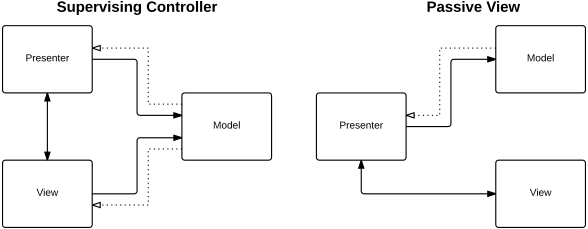
\includegraphics[width=0.5\textwidth]{mvp}
\caption{Supervising Controller and Passive View}
\label{fig:mvp}
\end{figure}

The \textbf{Supervising Controller} approach splits the User Interface in two components: a \emph{Presenter} and \emph{View} – like the classical MVP approach. The \emph{Model} can communicate changes to the \emph{View} using an Observer pattern (indirectly shown as dotted lines in Figure \ref{fig:mvp}). The \emph{View} can make direct changes to the model. In most cases this is done by simple mappings and \emph{Data Binding} capabilities provided by UI frameworks. Any user input is handled by the \emph{Presenter}. It determines how those interactions affect the underlying \emph{Model}. In addition, it handles complex view logic operations i.e. to prepare the model data for the view layer or vice versa, to transform the user input to fit the model requirements.

In contrast to the Supervising Controller, the \textbf{Passive View} totally separates the \emph{View} from the \emph{Model}. There is no direct or indirect interaction between them -- see Figure \ref{fig:mvp}. Interactions between \emph{View} and \emph{Model} is done exclusively via the \emph{Presenter}. This approach reduces the \emph{View} to an absolute minimum by using the \emph{Presenter} to handle all user input events, to update the \emph{Model} based on user interactions as well as to channel \emph{Model} changes back to the \emph{View}. As a result, the \emph{View} is made completely passive and is no longer responsible for updating itself from the \emph{Model}.

The primary driver for \emph{Passive View} is testing. This concept allows testing to be focused on the \emph{Presenter} without needing any interaction with the chosen UI framework.




\section{Android App Prototype}

\IEEEPARstart{T}{he} prototypical Android app, developed for this paper, is a simple weather app. It is able to show the current weather data for a location including temperature, humidity and wind. For retrieving this data, the app connects to the remote \emph{application programming interface} (API) of \emph{openweathermap.org}, a free-to-use service for retrieving weather data. The app also manages a list of favourite locations. Locations can either be specified using a free-text search field or by pointing locations on a map, for which the \emph{Google Maps} API was used.

\subsection{App Structure}

As mentioned above, the basic building blocks of an Android application are \emph{Activities}, \emph{Fragments} and \emph{Intents}. Applying MVP to an Android application therefore means to put attention on those components.

The implementation of MVP in the app prototype, follows the approach of Leiva \cite{AntLeiv14}, in which \emph{Activities} implement the view part. This means that in addition to extending the base Android \texttt{Activity} class, an activity class must also implement a \texttt{View} interface. The class structure around such an activity is illustrated in Fig. \ref{fig:androidmvp}.

\begin{figure}[h]
\centering
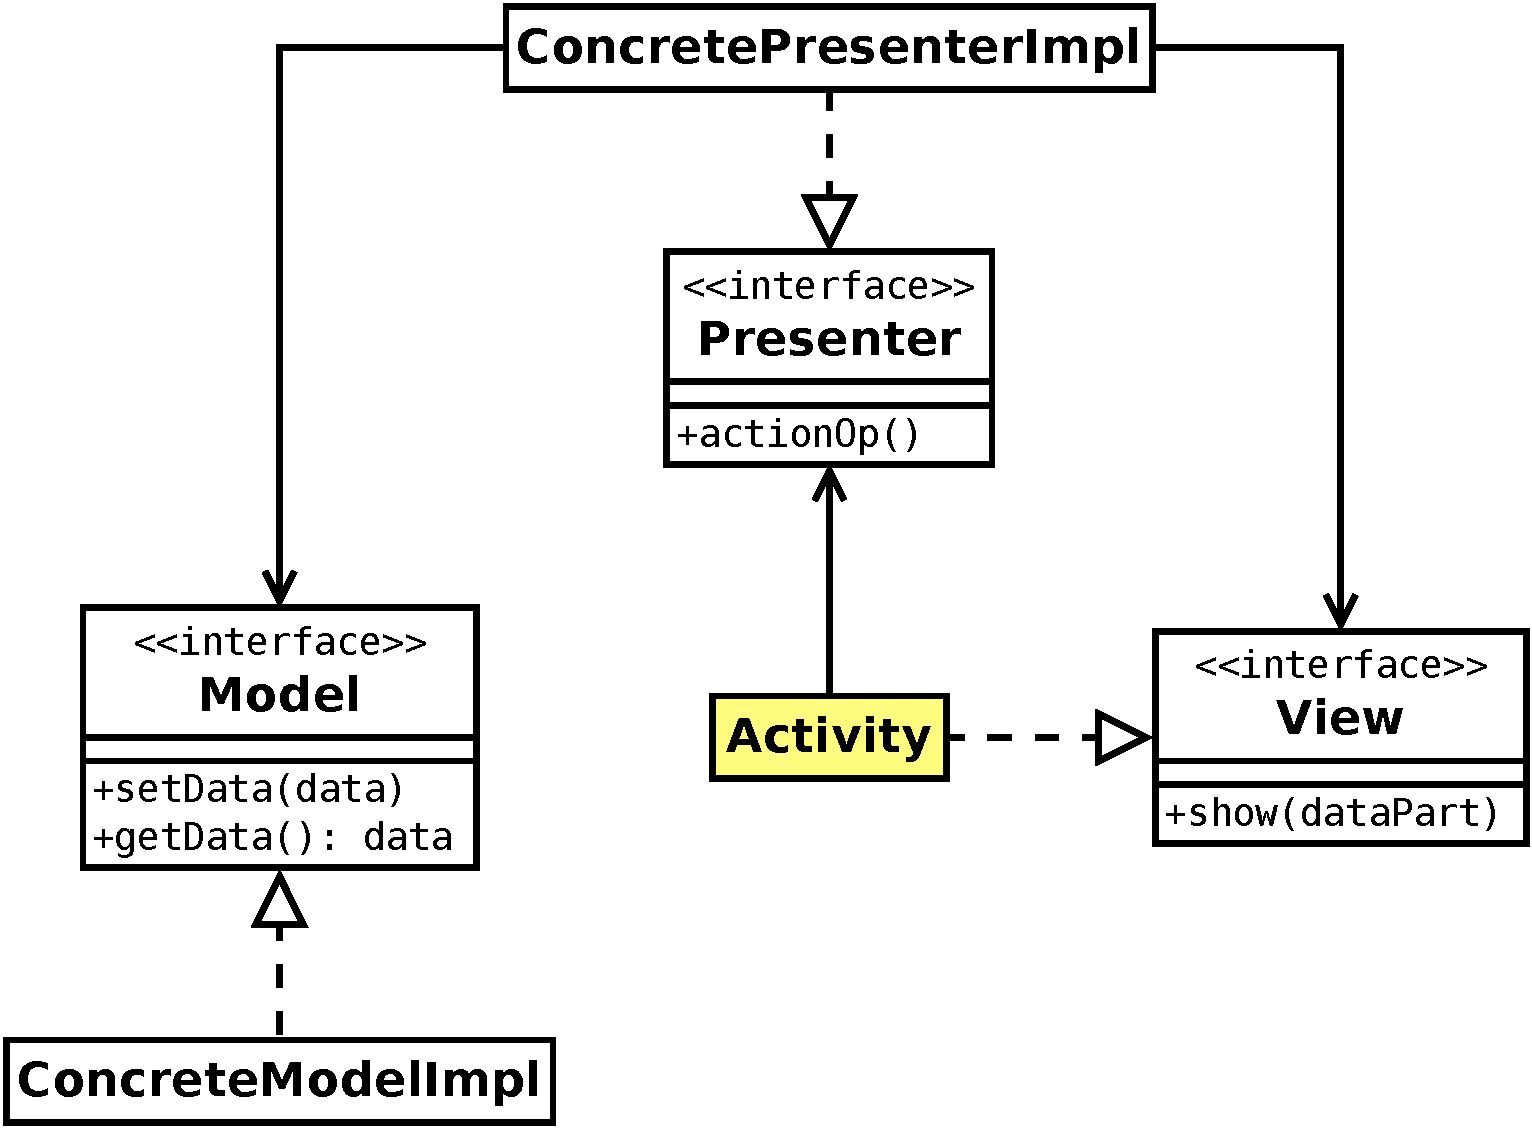
\includegraphics[width=0.45\textwidth]{diag1.pdf}
\caption{Class structure of an activity (highlighted with yellow background) in the context of an MVP architecture}
\label{fig:androidmvp}
\end{figure}

Each activity object has a presenter object associated, implementing the \texttt{Presenter} interface. On the other hand, the presenter object has a reference to the activity object. View related actions, like a click on a button, cause handler functions inside the \texttt{Activity} class being called. Those handler functions do nothing more than executing corresponding actions on the presenter object.

The interaction with the model is done only by the presenter. This makes the app prototype an implementation of the \emph{Passive View} kind of MVP.
An example of an interaction sequence between objects of \texttt{Activity}, \texttt{Presenter} and \texttt{Model} classes is shown in Fig. \ref{fig:androidmvpseq}. Clicking on a button -- let's assume it's labeled \emph{Refresh} -- causes the handler function in the \texttt{Activity} being called. An action is executed on the presenter object by the activity. The presenter retrieves new data from the model and afterwards calls the activity (the \texttt{View}) for showing that data.

\begin{figure}[h]
\centering
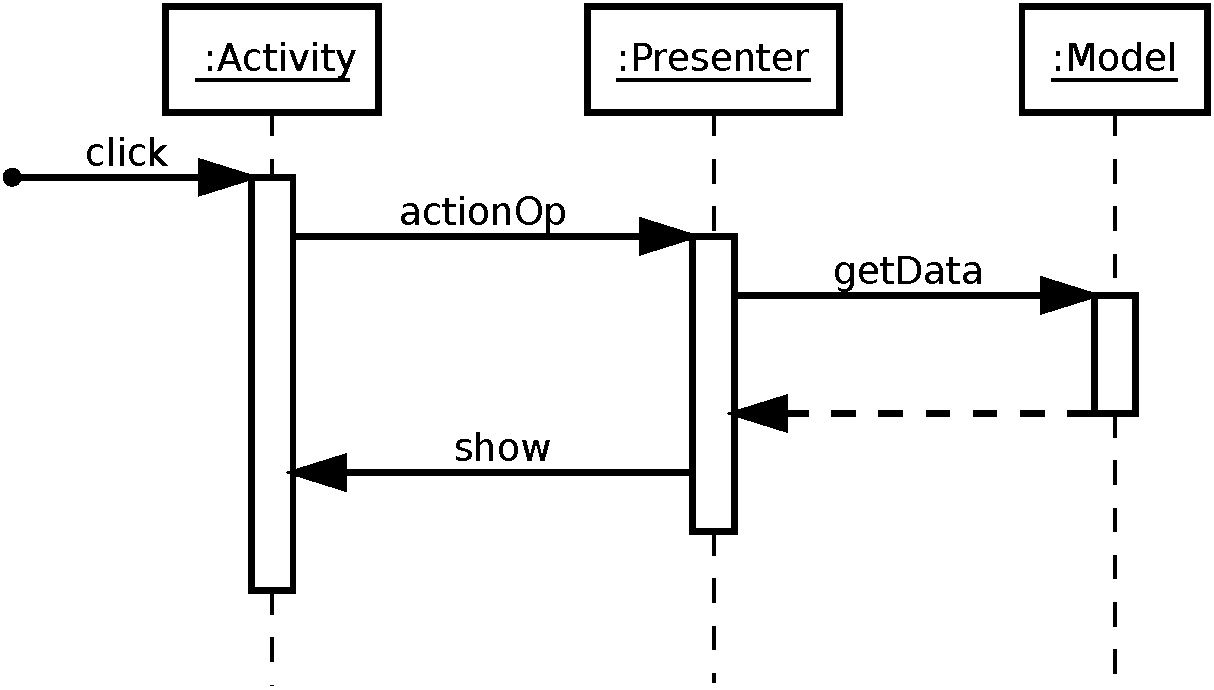
\includegraphics[width=0.45\textwidth]{diag2.pdf}
\caption{Interaction sequence involving objects of \texttt{Activity}, \texttt{Presenter} and \texttt{Model} classes}
\label{fig:androidmvpseq}
\end{figure}

For model operations that take a while to execute -- like retrieving weather data from \emph{openweathermap.org}, which can take a few seconds -- the interaction between presenter and model was implemented in an asynchronous way. Model objects, used by multiple presenters, additionally implement the \emph{Observer} design pattern (see \cite[p. 287]{GangOfFour}) to notify all registered presenters on model changes.

The MVP pattern can be applied to \emph{Fragments} the same way as it is described above for \emph{Activities}. Presenters of \emph{Fragment} objects most likely share their model with other \emph{Fragments} and other \emph{Activities}. An example of this was implemented in the \texttt{WeatherDetailsActivity} of the app prototype, which shows the weather data for a selected location. The part of the view showing temperature and wind information was extracted into a separate \emph{Fragment} with its own presenter implementation. Clicking on the \emph{Refresh} button causes the presenter of the activity to instruct the model to fetch updated weather data from \emph{openweathermap.org}. When this data is available, the model notifies all registered observers -- in this case the presenter of the activity and the presenter of the fragment. Both presenters go back to the corresponding view objects and cause the updated data to be displayed.

As \emph{Intents} are received by the activity object, they can be handled like any other view-related action (e.g. a click on a button). Whenever an intent was received by the activity, a corresponding action on the presenter object is executed -- nothing else. When it comes to creating intents, e.g. for switching to another activity, things get a bit more complicated. One would typically do such action inside the presenter, but intents require to be sent from a specific context, which can either be an activity or the application itself. This means that for creating an intent, the presenter must either address the main application object directly or go back to the activity and let the activity send the intent.

This answers RQ3, showing that MVP can be applied to an Android application considering the \emph{Activity}, \emph{Fragment} and \emph{Intent} building blocks.

As an additional remark, the usage of the \emph{Dependency Injection} (see \cite{FowlerIoC}) library \emph{Dagger} should be mentioned. The library was used to resolve object dependencies, like the one which exists between an \texttt{Activity} and an \texttt{Presenter} object (and vice versa). It automatically injects references of both objects into each other.

\subsection{Testing the App}

As mentioned before in section \ref{sec:research}, a key benefit of an MVP architecture is the increased testability of the software.
To demonstrate this ability, some tests for the app prototype were created using the testing capabilities of the Android SDK -- the Android testing framework:

\textbf{Activity Unit Test}:
An activity object will be created in an isolated environment. This means that, except from the tested activity object, every other component, like the application itself, is replaced by a mock implementation. This includes the presenter object as well. Using such a mock presenter implementation allows to easily test the interaction between an activity and its presenter.
An example would be the simulation of a button click and the assertion, if the presenter object was called correctly.
Without having MVP in place, the isolation of an activity object would be way more complicated or may even not be possible at all.

\textbf{Model Unit Test}
As the model objects of the app prototype have no dependency to any Android related component, they are very good for being tested through unit tests. As described for activities above, the model object will be created in an isolated environment with a mock presenter implementation.



\section{Conclusion}

\IEEEPARstart{I}{n} course of this research paper we have analyzed the characteristics given by the \emph{Android} SDK and have identified 
principle components which are generally used for developing \emph{Android} applications. Those components have been examined regarding their composition and characteristics. 
Finally we can offer an MVP approach for \emph{Android} and a corresponding prototype app demonstrating how principle \emph{Android} components can be structured for applying MVP.

However, just the essential SDK components have been examined regarding their MVP compatibility and used in the prototype. 
The MVP pattern for \emph{Android} would only succeed in practice if a wide bandwidth of SDK components was adaptable. 
In course of additional research studies addressing this topic we recommend to examine further SDK components and 
evaluate them regarding their MVP compatibility by implementing prototypes.

There are further and particularly similar MVP approaches developed and provided by the \emph{Android} developer community. 
\emph{Google} developer \emph{Chris Banes} has developed the \emph{Android} app \emph{philm} basing on MVP. 
The very demonstrative source code is offered on \emph{github} [https://github.com/chrisbanes/philm] and worth seeing. 
Moreover there is a huge developer community on \emph{Google+} [https://plus.google.com/communities/114285790907815804707] dealing with different MVP approaches. 
Finally, we want to draw your attention to the paper \emph{Android Passive MVC: a Novel Architecture Model for Android Application Development} 
[Quelle] which is worth reading and has been an inspiration for our approach. Although the paper proposes an architecture which is rather MVC than MVP-based, 
it offers an interesting approach how the components of an \emph{Android} app can be organized for building an MV-x structure. 





% if have a single appendix:
%\appendix[Proof of the Zonklar Equations]
% or
%\appendix  % for no appendix heading
% do not use \section anymore after \appendix, only \section*
% is possibly needed

% use appendices with more than one appendix
% then use \section to start each appendix
% you must declare a \section before using any
% \subsection or using \label (\appendices by itself
% starts a section numbered zero.)
%


\appendices

% you can choose not to have a title for an appendix
% if you want by leaving the argument blank
%\section{}
%Appendix two text goes here.


% use section* for acknowledgement



% Can use something like this to put references on a page
% by themselves when using endfloat and the captionsoff option.
\ifCLASSOPTIONcaptionsoff
  \newpage
\fi



% trigger a \newpage just before the given reference
% number - used to balance the columns on the last page
% adjust value as needed - may need to be readjusted if
% the document is modified later
%\IEEEtriggeratref{8}
% The "triggered" command can be changed if desired:
%\IEEEtriggercmd{\enlargethispage{-5in}}

% references section

% can use a bibliography generated by BibTeX as a .bbl file
% BibTeX documentation can be easily obtained at:
% http://www.ctan.org/tex-archive/biblio/bibtex/contrib/doc/
% The IEEEtran BibTeX style support page is at:
% http://www.michaelshell.org/tex/ieeetran/bibtex/
%\bibliographystyle{IEEEtran}
% argument is your BibTeX string definitions and bibliography database(s)
%\bibliography{IEEEabrv,../bib/paper}
%
% <OR> manually copy in the resultant .bbl file
% set second argument of \begin to the number of references
% (used to reserve space for the reference number labels box)
\begin{thebibliography}{1}

\bibitem{PassiveMVC}
K. Sokolova, M. Lemercier, and L. Garcia: \emph{Android Passive MVC: a Novel Architecture Model for Android Application Development.} In: PATTERNS 2013, The Fifth International Conferences on Pervasive Patterns and Applications, p. 7-12, 2013.

\bibitem{GartnerAndroid2014}
Gartner: \emph{Gartner Says Worldwide Traditional PC, Tablet, Ultramobile and 
Mobile Phone Shipments Are On Pace to Grow 6.9 Percent in 2014}, March 2014, 
[Online]. http://www.gartner.com/newsroom/id/2692318 (retrieved 02-Dec-2014)

\bibitem{AppBrainStats}
App Brain: \emph{Android Statistics -- Number of Android applications}. 
[Online].
http://www.appbrain.com/stats/number-of-android-apps (retrieved 02-Dec-2014)

\bibitem{AndroidDeveloperCollection}
J. Steele, N. To, S. Conder, and L. Darcey: \emph{The Android Developer's Collection.} Addison-Wesley Professional, December 2011.

\bibitem{BallOfMud}
B. Foote and J. Yoder: \emph{Big Ball of Mud.} Addison-Wesley, 1997.

\bibitem{TaligentMVP}
M. Potel: \emph{MVP: Model-View-Presenter the taligent programming model for C++ and Java}, Taligent Inc., 1996.

\bibitem{GangOfFour}
E. Gamma, R. Helm, R. Johnson, and J. Vlissides: \emph{Design Patterns: Elements of Reusable Object-Oriented Software,} 1\textsuperscript{st} ed. Addison-Wesley Professional, November 1994.


%\bibitem{}
%H.~Kopka and P.~W. Daly, \emph{A Guide to \LaTeX}, 3rd~ed.\hskip 1em plus
%  0.5em minus 0.4em\relax Harlow, England: Addison-Wesley, 1999.


\end{thebibliography}

% biography section
% 
% If you have an EPS/PDF photo (graphicx package needed) extra braces are
% needed around the contents of the optional argument to biography to prevent
% the LaTeX parser from getting confused when it sees the complicated
% \includegraphics command within an optional argument. (You could create
% your own custom macro containing the \includegraphics command to make things
% simpler here.)
%\begin{biography}[{\includegraphics[width=1in,height=1.25in,clip,keepaspectratio]{mshell}}]{Michael Shell}
% or if you just want to reserve a space for a photo:

%\begin{IEEEbiography}{Michael Shell}
%Biography text here.
%\end{IEEEbiography}

% if you will not have a photo at all:
%\begin{IEEEbiographynophoto}{John Doe}
%Biography text here.
%\end{IEEEbiographynophoto} 

% insert where needed to balance the two columns on the last page with
% biographies
%\newpage

%\begin{IEEEbiographynophoto}{Jane Doe}
%Biography text here.
%\end{IEEEbiographynophoto}

% You can push biographies down or up by placing
% a \vfill before or after them. The appropriate
% use of \vfill depends on what kind of text is
% on the last page and whether or not the columns
% are being equalized.

%\vfill

% Can be used to pull up biographies so that the bottom of the last one
% is flush with the other column.
%\enlargethispage{-5in}



% that's all folks
\end{document}


